\subsection[Схема Блэкли]{Схема разделения секрета Блэкли}\index{схема разделения секрета!Блэкли|(}\index{схема разделения секрета!векторная|(}
\selectlanguage{russian}

Схема разделения секрета Блэкли (\langen{George Robert Blakley},~\cite{Blackley:1979}), также называемая векторной схемой, основывается на том, что для восстановления всех координат точки в $K$-мерном пространстве, принадлежащей нескольким неколлинеарным гиперплоскостям, необходимо и достаточно знать уравнения $K$ таких плоскостей. То есть в двумерном пространстве нужны две пересекающиеся прямые, в трёхмерном -- три пересекающиеся в нужной точке плоскости и так далее.

\begin{figure}[thb]
	\centering
	\subfloat{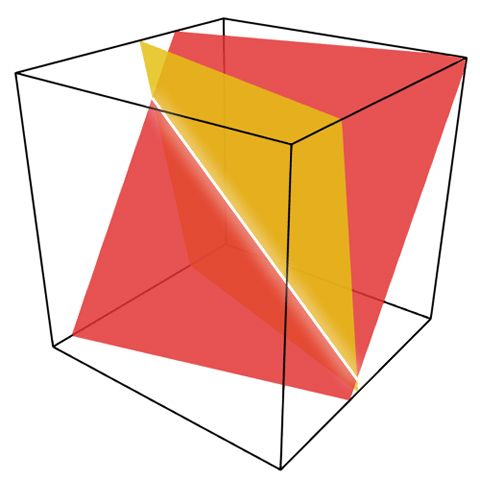
\includegraphics[width=0.45\textwidth]{pic/blakley-2}}
	~~~~
	\subfloat{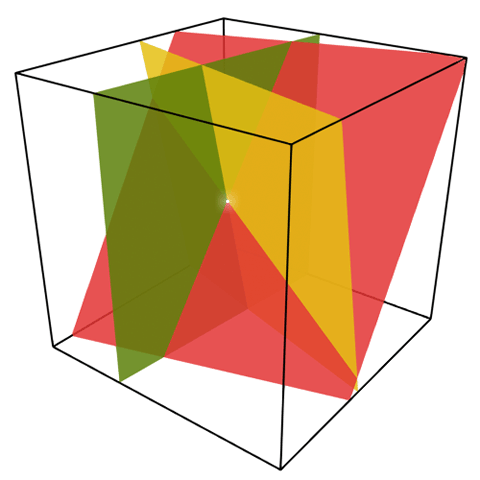
\includegraphics[width=0.45\textwidth]{pic/blakley-3}}
	\caption{Для восстановления координат точки пересечения плоскостей в трёхмерном пространстве необходимо и достаточно знать уравнения трёх таких плоскостей. Данные изображения приведены только для иллюстрации идеи -- в схеме Блэкли используется конечное поле, плоскости в котором сложно представить на графике. Рисунок участника English Wikipedia stib, доступно по \href{https://creativecommons.org/licenses/by-sa/3.0/deed.ru}{лицензии CC-BY-SA 3.0}}
\end{figure}

Для разделения секрета $M$ между $N$ сторонами таким образом, чтобы любые $K$ сторон могли восстановить секрет, доверенный центр выполняет следующие операции:
\begin{itemize}
	\item выбирает несекретное большое простое число $p$ ($p > M$);
	\item выбирает случайную точку, одна из координат которой (например, первая) будет равна разделяемому секрету M: $(x_1 = M, x_2, \dots, x_K)$;
	\item для каждого участника $i$ выбирает $K$ случайных коэффициентов гиперплоскости $C^i_1, C^i_2, \dots, C^i_{K}$ ($\ne 0$), а последний коэффициент $C^i_{K+1}$ вычисляется таким образом, чтобы гиперплоскость проходила через выбранную точку:
		\[ \begin{array}{l}
			C^i_1 x_1 + C^i_2 x_2 + \dots + C^i_K x_K + C^i_{K+1} = 0 \mod p, \\
			C^i_{K+1} = - ( C^i_1 x_1 + C^i_2 x_2 + \dots + C^i_K x_K ) \mod p; \\
		\end{array} \]
	\item раздаёт каждой стороне по следу в виде коэффициентов общего уравнения гиперплоскости $C^i_1, C^i_2, \dots, C^i_{K}, C^i_{K+1}$ и общему модулю $p$.
\end{itemize}

Если стороны могут собраться вместе и получить не менее чем $K$ различных гиперплоскостей, то составив и решив систему уравнений с $K$ неизвестными, они смогут получить все координаты точки $x_1, x_2, \dots, x_k$:

\[ \left\{ \begin{array}{l}
    C^1_1 x_1 + C^1_2 x_2 + \dots + C^1_K x_K + C^1_{K+1} = 0 \mod p, \\
    \dots, \\
    C^K_1 x_1 + C^K_2 x_2 + \dots + C^K_K x_K + C^K_{K+1} = 0 \mod p. \\
\end{array} \right. \]

Если собрано меньшее количество следов (уравнений гиперплоскостей), то их будет недостаточно для решения системы уравнений.

\example
Приведём пример разделения секрета по схеме Блэкли в $\GF{11}$. При разделении секрета $M$ используя $(3,N)$ схему Блэкли участники получили следы $(4, 8, 2, 6)$, $(2, 6, 8, 3)$, $(6, 8, 4, 1)$. Зная, что следы представляют собой коэффициенты в уравнении плоскости общего вида, а исходный секрет -- первую координату точки пересечения плоскостей, составляем систему уравнений для нахождения координаты этой точки:

\[ \left\{\begin{aligned}
   \left( 4\cdot x_1 + 8\cdot x_2 + 2\cdot x_3 + 6 \right) &= 0 &\mod 11,  \\
   \left( 2\cdot x_1 + 6\cdot x_2 + 8\cdot x_3 + 3 \right) &= 0 &\mod 11,  \\
   \left( 6\cdot x_1 + 8\cdot x_2 + 4\cdot x_3 + 1 \right) &= 0 &\mod 11.  \\
\end{aligned} \right. \]

Решением данной системы будет являться точка (6, 4, 2), а её первая координата -- разделяемый секрет.
\exampleend

\index{схема разделения секрета!векторная|)}\index{схема разделения секрета!Блэкли|)}
